% !TEX program = lualatex
\documentclass[a4paper,10pt]{article}
\usepackage{graphicx}
\usepackage{amsmath}
\usepackage{amssymb}
\usepackage{hyperref}
\usepackage{titlesec}
\usepackage{helvet}
\usepackage{parskip}
\usepackage{multicol}
\usepackage{fontspec}
\setmainfont{Futura}
\usepackage[inline, shortlabels]{enumitem}

\usepackage[margin=0.8in]{geometry}     % Overall page margins
\setlength{\columnsep}{2em}           % Space between columns
\setlength{\parskip}{0.5em}             % Space between paragraphs

\titleformat{\section}
  {\normalfont\small\bfseries}
  {\thesection.}{0.5em}{}
\titlespacing*{\section}
  {0pt}{0.5em}{0.4em}

  \titleformat{\subsection}[runin]
  {\normalfont\small\bfseries}
  {\thesubsection.}{0.5em}{}
\titlespacing*{\subsection}
  {0pt}{0.2em}{0.2em}

\setlist{nolistsep}
\setlist[itemize]{leftmargin=*}
\setlist[enumerate]{leftmargin=*}
\setlength{\textfloatsep}{5pt}

\begin{document}
\begin{center}
\Large Chatlocal: Retrieval Augmented Generation\\[0.8em]
\small Raoul Grouls, Marijn Siebel\\[0.4em]
\footnotesize HAN University of Applied Sciences\\[3em]
\end{center}

\begin{multicols}{2}
\section{Overview}
\subsection{Problem}
Talking with a modern Large Language Model (LLM) can be helpful. However, when you have private context such as personal documents, meeting minutes or project proposals, the LLM has no knowledge of this context. To solve this issue, it is posssible to manually copy-paste some of the context into the chat. But what if your context is a 100 pages, and you don't know exactly where the right context is you need to answer your question? And, in addition to that, you are concerned about privacy? 
\subsection{Solution}
Retrieval Augmented Generation is a technique that combines the best of both worlds: the LLM can generate text, but it can also retrieve context from a document collection. Chatlocal is a RAG solution that offers the user the flexibility to \begin{enumerate*}[a)]\item choose open source LLMs and \item to run everything on local hardware.\end{enumerate*} Upload your documents once, and the system will automatically retrieve relevant context when answering your questions. 
\section{Key Features}
\begin{itemize}
\item Just-in-time context retrieval from uploaded documents
\item Choice between commercial and open-source models
\item References with title and page number
\item Fully local deployment option
\item Upcoming: Direct source linking in frontend
\end{itemize}
\section{Upcoming Features}
\begin{itemize}
\item Direct source linking in frontend
\item Automated Knowledge Graph generation
\item Restricting query to a subset of documents
\end{itemize}
\section{Privacy}
Given proper hardware, it is possible to download open source LLMs for every step in the proces (both retrieval and generation).
This ensures that no data will ever leave your hardware.
The downside of this approach is that commercial models typically outperform open source models.
\section{Important Considerations}
\subsection{Context Understanding}\label{sec:context}
Because the system \textit{seems} to understand all of your context, a common misconception is that the system actually has an overview over your context. It does not!
The system operates like an student that is smart, but didnt study the material. It is just very fast at looking up one or two relevant pages like in an "open-book exam"
\subsection{Accuracy \& Limitations}
\begin{itemize}
	\item Hallucination is an risk inherent to \textbf{all} LLMs
	\item This can be mitigated through RAG, but not yet guaranteed, regardless of what LinkedIn tells you
	\item Source verification always recommended
	\item Complex cross-document queries may have reduced accuracy (due to \S~\ref{sec:context})
\end{itemize}

\section{Technical Architecture}
\begin{itemize}
\item Python with FastAPI framework
\item Ollama for open-source LLM hosting
\item OpenAI API integration (optional)
\item Document embedding via:
  \begin{itemize}
  \item SentenceTransformers
  \item Ollama nomic-embed
  \end{itemize}
\item ChromaDB for vector storage
\item HTML5, JavaScript, CSS
\end{itemize}
\section{Deployment Options}
\begin{itemize}
\item Most open source LLMs with acceptable performance need a minimum 32GB of RAM
\item A GPU is not necessary but speeds things up
\end{itemize}
\end{multicols}

% insert an image
\begin{figure*}[b]     % [t] for top of page, [b] for bottom
    \centering
    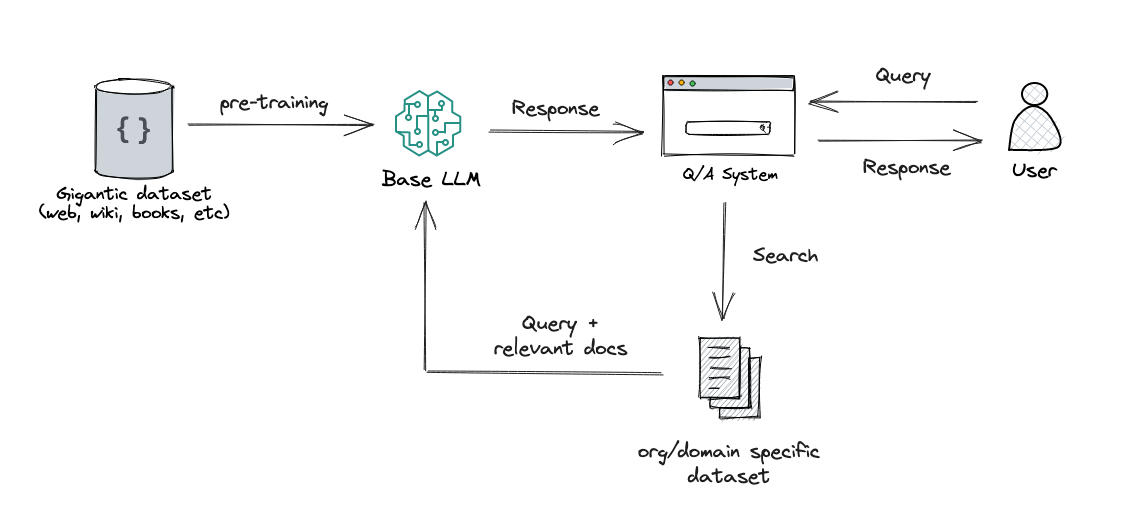
\includegraphics[width=0.9\textwidth]{rag.png}
\end{figure*}


\end{document}
